\chapter{Identifikasi Masalah dan Rancangan Solusi}

\newcommand{\ccnormspacing}{\baselineskip=12pt}
\newcommand{\ccnormspacingcenter}{\centering\arraybackslash\ccnormspacing}

Bab Identifikasi Masalah dan Rancangan Solusi berisi tentang penjelasan analisis permasalahan yang menjadi dasar dari tugas akhir ini. Secara garis besar, proses perancangan solusi akan mengikuti metodologi yang sudah ditetapkan yaitu pendekatan \textit{User-Centered Design} (UCD) menurut ISO 9241-210. Proses yang akan dibahas pada bab ini meliputi perancangan proses desain, identifikasi konteks penggunaan, analisis kebutuhan perangkat lunak, dan perancangan prototipe perangkat lunak. Gambaran alur UCD yang digunakan pada tugas akhir dapat dilihat pada Gambar \ref{fig:diagram_alur_kerja}.

\begin{figure}[h]
  \centering
  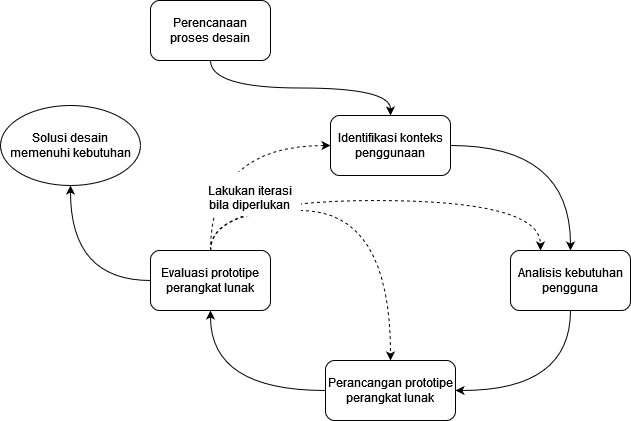
\includegraphics[width=0.8\textwidth]{chapter-1-method.png}
  \caption{Alur Kerja Penelitian}
  \label{fig:diagram_alur_kerja}
\end{figure}

\section{Perancangan Proses Desain}
\label{sec:perancangan_proses_desain}

Pada tahap perancangan proses desain dilakukan persiapan sumber daya yang diperlukan selama proses desain, serta penentuan ruang lingkup permasalahan.

% Sumber daya proses design

Ruang lingkup permasalahan yang ditentukan selama pengerjaan tugas akhir sebagai berikut

\begin{enumerate}
  \item Target Pengguna
  \subitem Target pengguna selama penelitian adalah pengguna \textit{smartphone} berbasis Android di Indonesia dengan rentang umur 18-34 tahun. Rentang usia tersebut adalah usia mayoritas pengguna media sosial di Indonesia. \parencite{mediasosial2020} 
  
  \item Fungsionalitas Aplikasi
  \subitem Lingkup fungsionalitas aplikasi adalah bagaimana desain interaksi yang baru dapat memperbaiki masalah yang ditemukan pada aplikasi Digital Wellbeing saat ini. Fungsionalitas dari aplikasi menyesuaikan dengan analisis hasil yang didapatkan dari riset dan wawancara. 
   
  \item Lingkup Pengembangan Aplikasi
  \subitem Desain interaksi aplikasi pencegah distraksi yang dibuat memiliki bentuk \textit{mobile interface} dengan mewujudkan sebuah prototipe aplikasi dalam \textit{platform Android}. Aplikasi Digital Wellbeing milik Google ditetapkan menjadi garis dasar pengembangan prototipe aplikasi tersebut.

\end{enumerate}

% * =======================================================================
% *   ||  ||  ||  ||  ||  ||  ||  ||  ||  ||  ||  ||  ||  ||  ||  ||  ||
% * =======================================================================


\section{Identifikasi Konteks Penggunaan}
\label{sec:identifikasi_konteks_penggunaan}

Pada tahap ini dilakukan proses analisis pengguna melalui data yang didapatkan dari ulasan pengguna aplikasi Digital Wellbeing dari situs Google Play Store, serta riset dengan metode wawancara. Kemudian akan dilakukan penyusunan persona pengguna dan pengidentifikasian fungsionalitas aplikasi yang akan membantu menentukan kebutuhan dan tujuan pengguna.

\subsection{Riset dan Analisis Pengguna}
\label{subsec:riset_analisis}

Tahap ini bertujuan untuk menganalis target pengguna, sehingga didapatkan data perilaku, masalah, tujuan, dan kebutuhan pengguna aplikasi Digital Wellbeing. Riset dilakukan dengan mengumpulkan data ulasan pengguna aplikasi Digital Wellbeing dari situs Google Play Store \textcite{dwplaystorereviews}. Metode pengumpulan data ini dipilih dengan alasan mengacu pada ISO 9241-210, bahwa informasi yang sudah tersedia dari suatu produk dapat dimanfaatkan untuk melakukan modifikasi atau peningkatan kualitas produk \parencite{iso9241-210:2010}, dalam hal ini informasi berbentuk ulasan pengguna.

Hasil terhadap analisis ulasan pengguna kemudian divalidasi dengan wawasan yang didapat dari wawancara. Karena pada data ulasan pengguna dari Google Play Store tidak terdapat informasi mengenai umur dan perilaku pengguna, wawancara dengan pengguna yang termasuk ke dalam lingkup permasalahan perlu dilakukan juga untuk mendapatkan wawasan mengenai perilaku pengguna. Perilaku pengguna berguna untuk menyusun persona pengguna.

\subsubsection{Ulasan Pengguna}
\label{subsubsec:ulasan_pengguna}

Berdasarkan situs Google Play Store per 13 April 2022, terdapat 609.005 ulasan untuk aplikasi Digital Wellbeing. Untuk menentukan jumlah \textit{sample size}, ditentukan \textit{confidence level} sebesar 95\%. Dikumpulkan data sebanyak 1000 ulasan dari target pengguna yang telah disebutkan pada bab \ref{sec:identifikasi_konteks_penggunaan},  kemudian dikategorikan secara manual, lalu didapatkan 288 ulasan yang dapat digunakan untuk menyusun masalah pengguna, sehingga \textit{sample} data memiliki \textit{margin of error} sebesar 5.78\%.

Pengkategorian ulasan dilakukan secara manual sehingga menghasilkan 11 kategori. Rincian tentang kategori tersebut dapat dilihat pada tabel \ref{tab:daftar_kategori}.

\RaggedLeft
\begin{small}
\begin{longtable}[c]{|W{c}{0.08\textwidth}|>{\ccnormspacing}m{0.72\textwidth}|>{\ccnormspacingcenter}m{0.1\textwidth}|}
  \caption{Daftar Kategori Ulasan}
  \label{tab:daftar_kategori} \\
  \hline \rowcolor[HTML]{A3E5F5} \textbf{ID} & \centering\textbf{Kategori Ulasan} & \textbf{Jumlah Ulasan} \\ \hline \endfirsthead
  \hline \rowcolor[HTML]{A3E5F5} \textbf{ID} & \centering\textbf{Kategori Ulasan} & \textbf{Jumlah Ulasan} \\ \hline \endhead
  
  \hline \endfoot
  
  KU-01    & Kurangnya widget untuk menampilkan data di Home Screen & 63 \\ \hline
  KU-02    & Perlu dikembangkannya fitur laporan penggunaan aplikasi untuk menampilkan data & 47 \\ \hline
  KU-03    & Perlu dikembangkannya fitur Focus Mode dengan menambah keketatan & 47 \\ \hline
  KU-04    & Perlu dikembangkannya kemampuan penjadwalan untuk fitur App Timer dan Focus Mode & 36 \\ \hline
  KU-05    & Kurangnya fitur pengaturan tingkat keketatan untuk fitur-fitur & 29 \\ \hline
  KU-06    & Kurangnya kemampuan penundaan untuk fitur App Timer & 18 \\ \hline
  KU-07    & Perlu dikembangkannya fitur Bedtime Mode dengan menambah keketatan & 12 \\ \hline
  KU-08    & Kurangnya penjelasan atau susunan kata yang dapat memotivasi pengguna untuk memakai fitur-fitur aplikasi & 12 \\ \hline
  KU-09    & Kurangnya fitur pengelompokkan aplikasi & 11 \\ \hline
  KU-10    & Kurangnya fitur pengaturan jam untuk akhir sebuah hari & 7 \\ \hline
  KU-11    & Kurangnya fitur \textit{whitelisting} untuk pembatasan akses aplikasi oleh Focus Mode & 6 \\ \hline
\end{longtable}
\end{small}
\justifying
\FloatBarrier

Adapun sejumlah ulasan yang tidak tergolong dalam kategori dinilai tidak relevan dalam penyusunan masalah pengguna, dengan penjelasan sebagai berikut

\begin{enumerate}
  \item Ulasan yang menilai positif aplikasi tanpa menyebutkan adanya masalah yang ditemukan dari aplikasi
  \item Ulasan yang menilai negatif aplikasi tanpa menyebutkan masalah yang ditemukan dari aplikasi
  \item Ulasan yang menyebutkan adanya bug dari aplikasi, seperti tidak berfungsinya sebuah fitur di perangkat tertentu
  \item Ulasan yang menyebutkan masalah yang tidak termasuk ke dalam batasan tugas akhir
  \item Ulasan yang tidak dapat dimengerti, seperti huruf-huruf yang tersusun secara acak 
  \item Ulasan yang melaporkan bahwa aplikasi tidak dapat dihapus dari perangkat
\end{enumerate}

\subsubsection{Perilaku Pengguna}
Setelah melakukan analisis ulasan pengguna untuk aplikasi Digital Wellbeing, dilakukan wawancara untuk mendapatkan perilaku pengguna, memvalidasi masalah pengguna dari analisis ulasan, serta menemukan masalah lain yang tidak ditemukan dari ulasan. Target berjumlah 5 orang dengan kriteria sebagaimana telah dijelaskan pada subbab \ref{sec:perancangan_proses_desain}. Jumlah tersebut dipilih karena menurut \textcite{nielsenusabilityproblems}, penelitian dengan 5 orang responden sudah cukup untuk menemukan rata-rata 85\% masalah dari desain sebuah produk, dan menambah responden lebih banyak akan mendapatkan wawasan tambahan yang semakin sedikit.

 Data perilaku responden digunakan untuk menyusun persona pengguna, serta membantu menganalisis kebutuhan pengguna terkait aplikasi Digital Wellbeing. Sedangkan hasil validasi ulasan pengguna digunakan untuk  menggali inti masalah yang dikeluhkan. Kedua pengamatan tersebut akan dibahas lebih lanjut dalam analisis masalah, kebutuhan, dan tujuan pengguna. Rancangan pertanyaan dapat dilihat pada Lampiran \ref{chpt:daftar_pertanyaan_wawancara}. Detail pemetaan pengamatan dengan pertanyaan wawancara dapat dilihat pada Tabel \ref{tab:pemetaan_pengamatan_wawancara}

\RaggedLeft
\begin{small}
\begin{longtable}[c]{|>{\ccnormspacing}m{0.72\textwidth}|p{0.2\textwidth}|}
  \caption{Pemetaan Pengamatan dengan Pertanyaan Wawancara}
  \label{tab:pemetaan_pengamatan_wawancara} \\
  \hline \rowcolor[HTML]{A3E5F5} \multicolumn{1}{|c|}{\textbf{Pengamatan}} & \multicolumn{1}{|c|}{\textbf{No. Pertanyaan}} \\ \hline \endfirsthead
  \hline \rowcolor[HTML]{A3E5F5} \multicolumn{1}{|c|}{\textbf{Pengamatan}} & \multicolumn{1}{|c|}{\textbf{No. Pertanyaan}} \\ \hline \endhead

  \hline \endfoot
  
  \rowcolor[HTML]{DCF3FC} \multicolumn{2}{|l|}{\textbf{A. Perilaku Responden}} \\ \hline
  Identitas responden & 1, 2, 3 \\ \hline
  Perilaku penggunaan \textit{smartphone} responden & 4, 5, 6, 7, 8 \\ \hline
  Perilaku responden terkait aplikasi pencegah distraksi & 9, 10, 11, 12 \\ \hline
  Perilaku responden terkait aplikasi \textit{Digital Wellbeing} & 13, 14, 15 \\ \hline
  \rowcolor[HTML]{DCF3FC} \multicolumn{2}{|l|}{\textbf{B. Validasi Ulasan Aplikasi Digital Wellbeing}} \\ \hline
  Validasi masalah kurangnya fitur widget pada Homescreen & 16, 17, 18 \\ \hline
  Validasi masalah pada fitur laporan data penggunaan aplikasi pada \textit{smartphone} & 19 \\ \hline
  Validasi masalah pada fitur Focus Mode & 20, 21 \\ \hline
  Validasi masalah untuk kemampuan penjadwalan pada fitur-fitur & 22, 23, 24 \\ \hline
  Validasi masalah kurangnya fitur pengaturan tingkat keketatan & 25, 26, 27 \\ \hline
  Validasi masalah kurangnya fitur penundaan pada App Timer & 28, 29, 30 \\ \hline
  Validasi masalah pada fitur Bedtime Mode & 31, 32, 33 \\ \hline
  Validasi masalah kurangnya penjelasan dan susunan kata & 34, 35 \\ \hline
  Validasi masalah kurangnya fitur pengelompokkan aplikasi & 36 \\ \hline
  Validasi masalah kurangnya fitur pengaturan jam akhir hari & 37 \\ \hline
  Validasi masalah kurangnya kemampuan \textit{whitelisting} & 38 \\ \hline
\end{longtable}
\end{small}
\justifying
\FloatBarrier

Jumlah responden yang diwawancarai adalah 10 (sepuluh) orang. Data hasil wawancara dapat dilihat pada Lampiran \ref{chpt:hasil_wawancara}. Dari 10 responden, 90\% mengakui tujuan utama dari penggunaan smartphone adalah berkomunikasi melalui aplikasi \textit{messenger}, dengan tujuan sekunder yaitu berinteraksi dengan media sosial atau sebagai sarana hiburan. Ditemukan bahwa 4 dari 10 orang menggunakan \textit{smartphone} sebagai alat utama yang membantu dalam pekerjaan, dengan tujuan untuk berkomunikasi dengan rekan atau klien, menggunakannya sebagai \textit{workstation}, atau mencari ide dan inspirasi.

Dari wawancara, ditemukan bahwa seluruh responden mengakui distraksi terkait dengan \textit{smartphone} lebih banyak berasal dari luar \textit{smartphone} itu sendiri, yaitu dari keinginan diri sendiri menggunakan \textit{smartphone} untuk memenuhi tujuan sekunder mereka. Walaupun hanya 30\% responden yang mengeluhkan notifikasi dari \textit{smartphone} dianggap mendistraksi mereka dari kegiatan utama, 70\% mengakui perlu untuk mencegah distraksi dari notifikasi dengan cara menggunakan aplikasi pencegah distraksi atau mengubah pengaturan notifikasi aplikasinya secara langsung.

Ditemukan juga bahwa rata-rata durasi penggunaan \textit{smartphone} harian keseluruhan responden adalah 6.2 jam per hari, di mana 70\% responden dapat menggunakan \textit{smartphone} selama lebih dari 6 jam sehari. Kedua angka tersebut melebihi rata-rata durasi penggunaan \textit{smartphone} di Indonesia pada tahun 2021 yaitu 5.4 jam per hari \parencite{dataai2022smartphoneindonesia}.  Keseluruhan dari responden menilai skala rata-rata 4 (empat) dari 5 (lima) terhadap durasi penggunaan \textit{smartphone} harian mereka. Di antara seluruh responden, 70\% mengakui butuh bantuan dari sebuah aplikasi pencegah distraksi untuk menurunkan durasi penggunaan tersebut.

Selain untuk mengurangi durasi penggunaan, responden juga memerlukan bantuan sebuah aplikasi untuk melakukan hal lain yang berhubungan dengan perbaikan kebiasaan digital mereka. Ditemukan 50\% responden memerlukan bantuan aplikasi untuk memantau penggunaan \textit{smartphone}, baik secara keseluruhan atau per aplikasi, dalam merencanakan perbaikan digital mereka. Lalu, 80\% dari responden merasa perlu diingatkan tentang tugas / kegiatan yang harus diselesaikan saat mereka menggunakan \textit{smartphone}. Keberadaan sebuah pengingat dapat menyadarkan pengguna terhadap alasan mereka menggunakan aplikasi pencegah distraksi. Selain itu, 50\% dari responden juga menggunakan aplikasi untuk membantu dalam memperbaiki jadwal tidurnya. Mereka mengakui bahwa saat menggunakan \textit{smartphone} sebelum tidur, seringkali mereka tidak menyadari waktu sehingga melewati jadwal tidur mereka.

Wawasan tentang perilaku pengguna yang didapat dapat disusun dalam bentuk variabel-variabel perilaku yang berguna dalam pembentukan persona. \textcite{cooper2014face} menyarankan bahwa dalam menyusun variabel dapat ditemukan perbedaan yang cukup jelas jika fokus kepada tipe-tipe variabel berikut
\begin{enumerate}
  \item Aktivitas, yaitu apa yang dilakukan pengguna dan seberapa sering 
  \item Sikap, yaitu pendapat pengguna tentang domain produk dan teknologi
  \item Kemampuan, yaitu bakat pengguna dan kemampuan untuk belajar
  \item Motivasi, yaitu alasan keterlibatan pengguna pada domain produk 
  \item Keterampilan, yaitu kemampuan pengguna terkait domain produk dan teknologi
\end{enumerate}

Keseluruhan variabel perilaku pengguna dirangkum pada Tabel \ref{tab:perilaku_pengguna}

\RaggedLeft
\begin{small}
\begin{longtable}[c]{|W{c}{0.06\textwidth}|>{\ccnormspacing}m{0.66\textwidth}|>{\ccnormspacingcenter}m{0.175\textwidth}|}
  \caption{Daftar Variabel Perilaku Pengguna}
  \label{tab:perilaku_pengguna} \\
  \hline \rowcolor[HTML]{A3E5F5} \textbf{ID} & \multicolumn{1}{|c|}{\textbf{Variabel Perilaku Pengguna}} & \multicolumn{1}{|c|}{\textbf{Tipe Perilaku}} \\ \hline \endfirsthead
  \hline \rowcolor[HTML]{A3E5F5} \textbf{ID} & \multicolumn{1}{|c|}{\textbf{Variabel Perilaku Pengguna}} & \multicolumn{1}{|c|}{\textbf{Tipe Perilaku}} \\ \hline \endhead
  
  \hline \endfoot
  
  P-01  &  Menggunakan \textit{smartphone} dengan tujuan primer untuk berkomunikasi melalui aplikasi \textit{messenger}  & Aktivitas \\ \hline
  P-02  &  Menggunakan \textit{smartphone} dengan tujuan primer untuk membantu dalam pekerjaan & Aktivitas \\ \hline
  P-03  &  Menggunakan \textit{smartphone} dengan tujuan sekunder untuk berinteraksi lewat media sosial & Aktivitas \\ \hline
  P-04  &  Menggunakan \textit{smartphone} dengan tujuan sekunder sebagai sarana hiburan & Aktivitas \\ \hline
  P-05  &  Menilai skala rata-rata 4 (empat) dari 5 (lima) terhadap durasi penggunaaan \textit{smartphone} harian & Aktivitas \\ \hline
  P-06  &  Merasa sering terdistraksi oleh keinginan diri sendiri untuk menggunakan \textit{smartphone}  & Sikap \\ \hline
  P-07  &  Merasa sering terdistraksi oleh notifikasi dari \textit{smartphone} & Sikap \\ \hline
  P-08  &  Merasa \textit{smartphone} sebaiknya membatasi pengguna seminimal mungkin & Sikap \\ \hline
  P-09  &  Merasa perlu ada sebuah penghargaan jika berhasil mengikuti jadwal pembatasan \textit{smartphone} & Sikap \\ \hline
  P-10  &  Mampu membatasi diri dari menggunakan \textit{smartphone} tanpa bantuan & Kemampuan \\ \hline
  P-11  &  Ingin memblokir notifikasi aplikasi yang dinilai sebagai distraksi & Motivasi \\ \hline
  P-12  &  Ingin mengurangi durasi penggunaan \textit{smartphone} harian & Motivasi \\ \hline
  P-13  &  Ingin memantau kebiasaan penggunaan \textit{smartphone} & Motivasi \\ \hline
  P-14  &  Ingin dibantu mengingatkan diri terhadap tugas / aktivitas yang harus dilakukan & Motivasi \\ \hline
  P-15  &  Ingin mengingatkan diri terhadap jadwal tidur & Motivasi \\ \hline
  P-16  &  Ingin diingatkan ketika terlalu lama menggunakan aplikasi & Motivasi \\ \hline
  P-17  &  Ingin memblokir akses ke aplikasi yang dinilai mendistraksi tanpa menghapusnya & Motivasi \\ \hline
  P-18  &  Mampu mengatur jadwal kegiatan dengan baik sehingga tidak mudah terdistraksi & Keterampilan \\ \hline
  P-19  &  Terbiasa dalam mengoperasikan aplikasi pencegah distraksi pada \textit{smartphone}  & Keterampilan \\ \hline
\end{longtable}
\end{small}
\justifying
\FloatBarrier

\subsubsection{Masalah Pengguna}
\label{subsubsec:masalah_pengguna}

Ditemukan bahwa kategori ulasan yang didapat dari analisis ulasan pengguna cukup bervariasi dengan jumlah yang tersebar. Namun, ulasan pengguna tidak cukup dalam menggambarkan inti dari masalah yang mereka alami. Tahap verifikasi dari wawancara membantu menemukan inti masalah yang dikeluhkan serta gambaran utama dari keseluruhan masalah tersebut. Pengguna mengeluhkan bahwa mereka kurang dapat mendapat gambaran tentang kebiasaan digital yang baik dari aplikasi Digital Wellbeing. Selain itu, pengguna juga kesulitan dalam menggunakan aplikasi Digital Wellbeing secara efisien untuk mencapai tujuan-tujuannya.

Untuk menyelesaikannya, masalah tersebut perlu dipecahkan menjadi masalah-masalah pengguna yang dapat dirincikan. Hal tersebut dilakukan untuk mempermudah penentuan kebutuhan dan tujuan pengguna serta penyusunan solusi. Keseluruhan masalah pengguna dirangkum pada Tabel \ref{tab:daftar_masalah}.

\RaggedLeft
\begin{small}
\begin{longtable}[c]{|W{c}{0.08\textwidth}|>{\ccnormspacing}m{0.6\textwidth}|>{\ccnormspacingcenter}m{0.2\textwidth}|}
  \caption{Daftar Masalah Pengguna}
  \label{tab:daftar_masalah} \\
  \hline \rowcolor[HTML]{A3E5F5}
  \textbf{ID} & \centering\textbf{Masalah Pengguna} & \textbf{Keterkaitan} \\ \hline \endfirsthead
  \hline \rowcolor[HTML]{A3E5F5}
  \textbf{ID} & \centering\textbf{Masalah Pengguna} & \textbf{Keterkaitan} \\ \hline \endhead

  \hline \endfoot

  MP-01  & Pengguna kesulitan dalam melakukan pengaturan fitur-fitur aplikasi Digital Wellbeing secara efisien & KU-01, KU-04, KU-05, KU-09, KU-10, KU-11 \\ \hline
  MP-02  & Pengguna kesulitan dalam menganalisis kebiasaan digital diri lewat aplikasi Digital Wellbeing & KU-02 \\ \hline
  MP-03  & Pengguna merasa fitur-fitur aplikasi Digital Wellbeing kurang ketat dalam membantu memperbaiki kebiasaan digital & KU-03, KU-04, KU-05, KU-06, KU-07 \\ \hline
  MP-04  & Pengguna merasa fitur-fitur aplikasi Digital Wellbeing kurang fleksibel & KU-04, KU-06, KU-09, KU-10 \\ \hline
  MP-05  & Pengguna merasa interaksi dengan aplikasi Digital Wellbeing kurang pribadi & KU-08 \\ \hline
  MP-06  & Pengguna kurang dapat memahami penggunaan fitur-fitur yang disediakan oleh aplikasi Digital Wellbeing & KU-08 \\ \hline
  MP-07  & Pengguna kesulitan dalam mengakses informasi pada fitur-fitur aplikasi Digital Wellbeing & KU-01 \\ \hline
\end{longtable}
\end{small}
\justifying
\FloatBarrier

% $ =====================================================
% $   +  +  +  +  +  +  +  +  +  +  +  +  +  +  +  +  +
% $ =====================================================


\subsection{Persona}
\label{subsec:persona_pengguna}
Setelah dilakukan analisis mengenai perilaku dan masalah pengguna, dilakukan segmentasi pengguna menjadi beberapa kelompok persona. Persona merepresentasikan kelompok-kelompok pengguna dengan karakteristik dan perilaku yang berbeda. Persona berperan menjadi arah pengembangan interaksi aplikasi dan mengurangi kemungkinan mendesain aplikasi untuk semua orang sehingga menghasilkan desain yang tidak disenangi oleh siapapun. \parencite{cooper2014face}

\subsubsection{Pengelompokkan Awal Pengguna}
Tahap awal dalam menyusun persona adalah mengelompokkan pengguna-pengguna berdasarkan perannya. Dari 10 orang partisipan riset wawancara, dikelompokkan menjadi 3 peran berdasarkan kemampuannya dalam membatasi diri dari smartphone tanpa membutuhkan bantuan. Kemampuan ini dianalisis dari data-data yang didapat melalui wawancara, semakin tinggi tingkat kemampuannya berarti pengguna tersebut dapat membatasi dirinya dengan bantuan sesedikit mungkin.

Terdapat pengguna dengan kemampuan tingkat rendah beranggotakan 20\% partisipan, pengguna berkemampuan tingkat sedang sebanyak 30\%, dan pengguna dengan tingkat tinggi sebanyak 50\%. Maka dari itu, pembagian untuk kelompok pengguna adalah sebagai berikut
\begin{enumerate}
  \item Kelompok 1: Pengguna yang sangat memerlukan bantuan untuk membatasi diri dari \textit{smartphone} 
  \item Kelompok 2: Pengguna yang memerlukan bantuan ringan untuk membatasi diri dari \textit{smartphone}
  \item Kelompok 3: Pengguna yang tidak memerlukan bantuan untuk membatasi diri dari \textit{smartphone}
\end{enumerate}

\subsubsection{Pemetaan Kelompok Pengguna dengan Variabel Perilaku}
Setelah dilakukan pengelompokkan pengguna, variabel-variabel perilaku yang telah diidentifikasi pada tahap riset dan analisis pengguna perlu dipetakan ke setiap kelompok pengguna. Hal ini bertujuan untuk mengidentifikasi perilaku dari setiap kelompok untuk kemudian disusun personanya.

Variabel perilaku yang dipetakan ke masing-masing kelompok pengguna akan memiliki jenis nilai yang berbeda. Variabel perilaku seperti P-01 dan P-02 menunjukkan apa saja nilai perilaku yang dipenuhi kelompok pengguna tersebut. Variabel perilaku seperti P-10 dan P-19 menunjukkan rentang atau tingkat perilaku dari kelompok pengguna tersebut. Sedangkan variabel perilaku seperti P-08 dan P-09 menunjukkan apakah pengguna memiliki perilaku tersebut. Hasil dari proses pemetaan dapat dilihat pada Tabel \ref{tab:pemetaan_perilaku}.

\RaggedLeft
\begin{small}
\begin{longtable}[c]{|>{\ccnormspacing}m{0.10\textwidth}|>{\ccnormspacing}m{0.31\textwidth}|>{\ccnormspacingcenter}m{0.145\textwidth}|>{\ccnormspacingcenter}m{0.145\textwidth}|>{\ccnormspacingcenter}m{0.145\textwidth}|}
  \caption{Daftar Pemetaan Kelompok Pengguna dengan Variabel Perilaku}
  \label{tab:pemetaan_perilaku} \\
  \hline \rowcolor[HTML]{A3E5F5}
  \centering\textbf{Variabel Perilaku} & \centering\textbf{Deskripsi Perilaku} & \textbf{Kelompok 1} & \textbf{Kelompok 2} & \textbf{Kelompok 3} \\ \hline \endfirsthead
  \hline \rowcolor[HTML]{A3E5F5}
  \centering\textbf{Variabel Perilaku} & \centering\textbf{Deskripsi Perilaku} & \textbf{Kelompok 1} & \textbf{Kelompok 2} & \textbf{Kelompok 3} \\ \hline \endhead

  \hline \endfoot

  \centering P-10  & Mampu membatasi diri dari menggunakan \textit{smartphone} tanpa bantuan & Rendah & Sedang & Tinggi \\ \hline
  \centering P-01 P-02  & Tujuan primer menggunakan \textit{smartphone} & Komunikasi & Pekerjaan, Komunikasi & Komunikasi, Pekerjaan \\ \hline
  \centering P-03 P-04 & Tujuan sekunder menggunakan \textit{smartphone} & Hiburan, Media sosial & Hiburan, Media sosial & Hiburan, Media sosial \\ \hline
  \centering P-05 & Penilaian durasi penggunaan \textit{smartphone} harian berdasarkan skala 1-5 & 5 & 4 & 3 \\ \hline
  \centering P-06 P-07 & Sumber distraksi terkait \textit{smartphone} & Keinginan diri sendiri, \textit{smartphone}, pihak lain & Keinginan diri sendiri, \textit{smartphone}, pihak lain & Keinginan diri sendiri \\ \hline
  \centering P-18 & Keterampilan dalam menyusun jadwal kegiatan & Rendah & Tinggi & Sedang \\ \hline
  \centering P-19 & Kebiasaan dalam menggunakan aplikasi pencegah distraksi & Tinggi & Sedang & Sedang \\ \hline
  \centering P-08 & Merasa \textit{smartphone} sebaiknya membatasi pengguna seminimal mungkin &   & \textbf{V} & \textbf{V} \\ \hline
  \centering P-09 & Merasa perlu ada sebuah penghargaan jika berhasil mengikuti jadwal pembatasan \textit{smartphone} & \textbf{V} &   &   \\ \hline
  \centering P-11 & Ingin memblokir notifikasi aplikasi yang dinilai sebagai distraksi & \textbf{V} & \textbf{V} & \textbf{V} \\ \hline
  \centering P-12 & Ingin mengurangi durasi penggunaan smartphone harian & \textbf{V} & \textbf{V} & \textbf{V} \\ \hline
  \centering P-13 & Ingin memantau kebiasaan penggunaan smartphone & \textbf{V} & \textbf{V} & \textbf{V} \\ \hline
  \centering P-14 & Ingin dibantu mengingatkan diri terhadap tugas / aktivitas yang harus dilakukan & \textbf{V} & \textbf{V} &   \\ \hline
  \centering P-15 & Ingin mengingatkan diri terhadap jadwal tidur & \textbf{V} & \textbf{V} &   \\ \hline
  \centering P-16 & Ingin diingatkan ketika terlalu lama menggunakan aplikasi & \textbf{V} &   &   \\ \hline
  \centering P-17 & Ingin memblokir akses ke aplikasi yang dinilai mendistraksi tanpa menghapusnya & \textbf{V} &   &   \\ \hline

\end{longtable}
\end{small}
\justifying
\FloatBarrier

\subsubsection{Pemetaan Kelompok Pengguna dengan Masalah Pengguna}
Selain variabel perilaku, masalah pengguna pun perlu dipetakan dengan kelompok pengguna yang telah dibuat. Hal ini dilakukan untuk mengenali masalah yang dirasakan oleh kelompok pengguna spesifik, dan juga membantu dalam menyusun persona.

Ditemukan bahwa ketiga kelompok pengguna mengalami sebagian besar dari masalah pengguna yang ada. Masalah pengguna MP-03 di mana aplikasi Digital Wellbeing dinilai kurang ketat tidak dirasakan oleh kelompok pengguna 3 karena tingginya kemampuan dalam membatasi diri dari smartphone tanpa membutuhkan bantuan. Di sisi lain, masalah MP-04 tentang fleksibilitas aplikasi tidak dirasakan oleh kelompok pengguna 1 karena perilakunya yang menunjukkan kebutuhan atas keketatan tinggi dari aplikasi dalam membatasi penggunaan smartphone. Selain itu, akibat keterampilan kelompok pengguna 1 dalam menggunakan aplikasi pencegah distraksi, mereka tidak mengalami masalah MP-06 karena mereka sudah cukup mengerti fitur-fitur yang digunakan. Hasil dari proses pemetaan dapat dilihat pada Tabel \ref{tab:pemetaan_masalah}.

\RaggedLeft
\begin{small}
\begin{longtable}[c]{|>{\ccnormspacing}m{0.08\textwidth}|>{\ccnormspacing}m{0.31\textwidth}|>{\ccnormspacingcenter}m{0.145\textwidth}|>{\ccnormspacingcenter}m{0.145\textwidth}|>{\ccnormspacingcenter}m{0.145\textwidth}|}
  \caption{Daftar Pemetaan Kelompok Pengguna dengan Masalah Pengguna}
  \label{tab:pemetaan_masalah} \\
  \hline \rowcolor[HTML]{A3E5F5}
  \centering\textbf{ID} & \centering\textbf{Deskripsi Masalah} & \textbf{Kelompok 1} & \textbf{Kelompok 2} & \textbf{Kelompok 3} \\ \hline \endfirsthead
  \hline \rowcolor[HTML]{A3E5F5}
  \centering\textbf{ID} & \centering\textbf{Deskripsi Masalah} & \textbf{Kelompok 1} & \textbf{Kelompok 2} & \textbf{Kelompok 3} \\ \hline \endhead

  \hline \endfoot

  \centering MP-01 & Pengguna kesulitan dalam melakukan pengaturan fitur-fitur aplikasi Digital Wellbeing secara efisien & \textbf{V} & \textbf{V} & \textbf{V} \\ \hline
  \centering MP-02 & Pengguna kesulitan dalam menganalisis kebiasaan digital diri lewat aplikasi Digital Wellbeing & \textbf{V} & \textbf{V} & \textbf{V} \\ \hline
  \centering MP-03 & Pengguna merasa fitur-fitur aplikasi Digital Wellbeing kurang ketat dalam membantu memperbaiki kebiasaan digital & \textbf{V} & \textbf{V} &  \\ \hline
  \centering MP-04 & Pengguna merasa fungsionalitas fitur-fitur aplikasi Digital Wellbeing kurang fleksibel &  & \textbf{V} & \textbf{V} \\ \hline
  \centering MP-05 & Pengguna merasa interaksi dengan aplikasi Digital Wellbeing kurang pribadi & \textbf{V} & \textbf{V} & \textbf{V} \\ \hline
  \centering MP-06 & Pengguna kurang dapat memahami penggunaan fitur-fitur yang disediakan oleh aplikasi Digital Wellbeing &  & \textbf{V} & \textbf{V} \\ \hline
  \centering MP-07 & Pengguna kesulitan dalam mengakses informasi pada fitur-fitur aplikasi Digital Wellbeing & \textbf{V} & \textbf{V} & \textbf{V} \\ \hline

\end{longtable}
\end{small}
\justifying
\FloatBarrier

\subsubsection{Penyusunan Karakteristik Persona}
Setelah dilakukan pemetaan kelompok pengguna terhadap variabel perilaku dan masalah, kelompok pengguna tersebut dapat disusun menjadi persona yang utuh dengan diberikan identitas dan karakter dalam bentuk sebuah narasi. Di dalam narasi tersebut, garis besar hasil pemetaan juga perlu disebutkan ulang. Hal-hal tersebut dapat membuat persona terasa hidup sehingga mempermudah proses penentuan kebutuhan dan tujuan pengguna, serta pembuatan solusi desain.

\newpage
Berikut adalah hasil penyusunan karakteristik persona untuk ketiga kelompok pengguna

\begin{enumerate}
  \item Persona 1: Nico
  \subitem Nico adalah seorang mahasiswa berumur 21 tahun yang sedang menjalani semester akhir di universitasnya. Nico mengerjakan tugas akhir pada laptopnya, namun ia merasa mudah terdistraksi oleh \textit{smartphone}nya, baik dari keinginannya untuk memeriksa media sosial atau permainan, maupun notifikasi yang sering muncul. Oleh karena itu, Nico menggunakan aplikasi Digital Wellbeing untuk memblokir akses ke aplikasi yang ia rasa mendistraksi serta mematikan notifikasinya. Namun terkadang Nico membuka blokirnya terlalu sering sehingga dia merasa adanya fitur dari Digital Wellbeing tidak berpengaruh dalam membantunya mencegah distraksi dari \textit{smartphone}-nya. Nico merasa butuh bantuan yang cukup besar dalam mengendalikan dirinya terkait \textit{smartphone} karena ia sering menyadari bahwa dirinya terlalu sering menggunakan \textit{smartphone}, melupakan tugasnya, dan jadwal tidurnya pun terganggu.

  \item Persona 2: Maya
  \subitem Maya adalah seorang pegawai swasta berumur 28 tahun. Dalam kesehariannya, Maya menggunakan \textit{smartphone} untuk berkomunikasi dengan rekan kerjanya, membantu dalam pekerjaannya, dan sebagai hiburan di jam istirahat. Maya sering terdistraksi di jam kerjanya oleh notifikasi atau keinginannya untuk memeriksa \textit{smartphone}, sehingga menggunakan aplikasi Digital Wellbeing untuk memblokirnya. Maya menemukan fitur-fitur menarik lain yang ia rasa dapat membantu mencegah distraksi, dan menganalisa serta memperbaiki kebiasaan penggunaan \textit{smartphone}nya. Namun Maya merasa bahwa beberapa fitur dari Digital Wellbeing kurang fleksibel untuk menyesuaikan dengan jadwal kerjanya yang bervariasi, seperti kurangnya kemampuan membuat jadwal lebih dari satu. Maya juga merasa pengalaman yang dirasakan kurang cukup personal untuk cukup memotivasinya karena pesan pengingat yang ia dapatkan terlalu membosankan.

  \item Persona 3: Nathan
  \subitem Nathan adalah seorang lulusan baru dan pekerja yang berumur 23 tahun. Dia terbiasa dalam mengatur jadwal pekerjaannya, dan sesekali menyelipkan jadwal untuk beristirahat. Ia melakukan sebagian besar pekerjaannya menggunakan \textit{smartphone}, seperti berkomunikasi, mengatur jadwal, dan menulis catatan. Nathan sesekali merasa bahwa dirinya memeriksa media sosial di \textit{smartphone} di waktu yang tidak tepat di saat jadwal kerjanya. Maka Nathan menggunakan fitur Focus Mode dari Digital Wellbeing untuk mengingatkan dirinya jika akan bermain \textit{smartphone} di jam kerjanya dan memblokir notifikasi dari aplikasi-aplikasi yang dianggap mendistraksi. Namun, Nathan tidak menggunakan fitur lain dari Digital Wellbeing karena ia merasa tidak perlu bantuan cukup banyak, tampilan dari aplikasi tidak cukup menarik, dan fitur-fitur yang ada tidak memiliki deskripsi yang jelas atau pengaturan yang cukup mudah.

\end{enumerate}

\subsubsection{Pemilihan Tipe Persona}
Dari persona-persona yang telah disusun, perlu dipilih sebuah persona primer. Persona primer akan dijadikan target utama atau panduan dalam membuat desain solusi. Persona primer yang dipilih harus dipertimbangkan agar tidak mengecewakan persona-persona lainnya. Dalam hal ini, persona 2, Maya, akan dijadikan sebagai persona primer. Namun dipilih juga persona 1, Nico, sebagai persona sekunder agar desain solusi yang dibuat tetap mampu memenuhi kebutuhannya.

Keputusan ini diambil melihat pertimbangan bahwa salah satu masalah terbesar dari aplikasi Digital Wellbeing adalah sulitnya pengguna dalam menggunakan aplikasi secara efisien untuk mencapai tujuan-tujuannya. Masalah tersebut tercerminkan dari masalah-masalah yang dikeluhkan oleh persona Maya dan persona lainnya. Dalam hal itu, solusi yang didesain untuk persona Maya diharapkan dapat menyelesaikan masalah-masalah yang dialami persona lain. Di sisi lain, kebutuhan persona Nico atas bantuan untuk membatasinya dari smartphone perlu dipertimbangkan dalam solusi desain, tanpa mengganggu desain yang ditujukan untuk persona primer.

% $ =====================================================
% $   +  +  +  +  +  +  +  +  +  +  +  +  +  +  +  +  +
% $ =====================================================


\subsection{Analisis Fungsionalitas Aplikasi}
\label{subsec:analisis_fungsionalitas}

% TODO lengkapin fungsionalitas aplikasi pencegah distraksi yang umum

Dalam mengidentifikasi konteks penggunaan produk, penting untuk mengerti lingkungan sistem dari produk tersebut. Fungsionalitas dari aplikasi Digital Wellbeing dapat langsung dari aplikasinya. Keseluruhan fungsionalitasnya dapat telah dijabarkan dalam Tabel \ref{tab:daftar_fungsionalitas_app_dw}.
% > Dalam mengidentifikasi konteks penggunaan produk, penting untuk mengerti lingkungan sistem dari produk tersebut. Untuk aplikasi Digital Wellbeing, perlu diidentifikasi fungsionalitas dari aplikasi pencegah distraksi pada umumnya untuk membantu mengidentifikasi kebutuhan pengguna. Dalam Tabel \ref{tab:daftar_fungsionalitas_app_dw} terdapat fungsionalitas dari aplikasi Digital Wellbeing yang sudah diterapkan.
% Sementara dalam Tabel \ref{daftar_fungsionalitas_app_umum} terdapat fungsionalitas yang belum diterapkan dalam aplikasi Digital Wellbeing yang ditemukan dalam aplikasi pencegah distraksi lain yang telah dipelajari sebagai bagian dari studi literatur Bab \ref{studi_kasus_aplikasi}.

\RaggedLeft
\begin{small}
\begin{longtable}[c]{|W{c}{0.08\textwidth}|>{\ccnormspacing}m{0.82\textwidth}|}
  \caption{Daftar Fungsionalitas Aplikasi Digital Wellbeing}
  \label{tab:daftar_fungsionalitas_app_dw} \\
  \hline \rowcolor[HTML]{A3E5F5} \textbf{ID} & \multicolumn{1}{|c|}{\textbf{Fungsionalitas}} \\ \hline \endfirsthead
  \hline \rowcolor[HTML]{A3E5F5} \textbf{ID} & \multicolumn{1}{|c|}{\textbf{Fungsionalitas}} \\ \hline \endhead
  
  \hline \endfoot
  
  FD-01  &  Aplikasi dapat melacak penggunaan harian dari \textit{smartphone} atau suatu aplikasi, dari sisi durasi penggunaan, jumlah pembukaan, dan notifikasi yang diterima \\ \hline
  FD-02  &  Aplikasi dapat menampilkan laporan penggunaan \textit{smartphone} atau suatu aplikasi dalam bentuk grafik dan daftar \\ \hline
  FD-03  &  Pengguna dapat menyetel batas waktu per hari akses suatu aplikasi \\ \hline
  FD-04  &  Aplikasi dapat memberikan notifikasi terkait batas waktu akses suatu aplikasi \\ \hline
  FD-05  &  Aplikasi dapat memblokir akses terhadap suatu aplikasi \\ \hline
  FD-06  &  Aplikasi dapat memblokir notifikasi yang dikirim suatu aplikasi \\ \hline
  FD-07  &  Pengguna dapat mengatur jadwal aktivasi pemblokiran akses untuk aplikasi yang dipilih \\ \hline
  FD-08  &  Pengguna dapat menunda pemblokiran akses sebuah aplikasi secara sementara \\ \hline
  FD-09  &  Pengguna dapat mengatur jadwal aktivasi mode waktu tidur \textit{smartphone} \\ \hline
  FD-10  &  Pengguna dapat menunda sementara aktivasi mode tidur \\ \hline
  FD-11  &  Pengguna dapat membuka pengaturan notifikasi aplikasi \\ \hline
\end{longtable}
\end{small}
\justifying
\FloatBarrier

\subsection{Analisis Kebutuhan dan Tujuan Pengguna}
\label{subsec:analisis_kebutuhan_tujuan}

Bagian dari identifikasi konteks penggunaan ini akan menganalisis tentang kebutuhan serta tujuan dari pengguna mengenai aplikasi Digital Wellbeing dan aplikasi pencegah distraksi secara umum, dibantu dengan data dari perilaku dan persona pengguna, masalah pengguna, dan fungsionalitas aplikasi. Keduanya akan berguna dalam merancang perbaikan desain interaksi yang diperlukan dari aplikasi Digital Wellbeing, terutama untuk menyusun \textit{usability goals} dan \textit{user experience goals}.

\subsubsection{Kebutuhan Pengguna}
\label{subsubsec:kebutuhan_pengguna}

Kebutuhan pengguna adalah hal apa saja yang diperlukan pengguna untuk mencapai tujuannya dalam memakai aplikasi Digital Wellbeing. Analisis kebutuhan pengguna melibatkan masalah pengguna serta perilaku pengguna yang telah dibahas sebelumnya. Penjelasan kebutuhan pengguna dirangkum di dalam Tabel \ref{tab:daftar_kebutuhan}.

\RaggedLeft
\begin{small}
\begin{longtable}[c]{|W{c}{0.07\textwidth}|>{\ccnormspacing}m{0.67\textwidth}|>{\ccnormspacingcenter}m{0.17\textwidth}|}
  \caption{Daftar Kebutuhan Pengguna}
  \label{tab:daftar_kebutuhan} \\
  \hline \rowcolor[HTML]{A3E5F5}
  \textbf{ID} & \centering\textbf{Kebutuhan Pengguna} & \textbf{Keterkaitan} \\ \hline \endfirsthead
  \hline \rowcolor[HTML]{A3E5F5}
  \textbf{ID} & \centering\textbf{Kebutuhan Pengguna} & \textbf{Keterkaitan} \\ \hline \endhead

  \hline \endfoot

  K-01  & Pengalaman pengaturan fitur yang lebih efisien dengan kemampuan seperti pencarian dan pengelompokan aplikasi & MP-01 \\ \hline
  K-02  & Widget untuk mengakses data serta melakukan pengaturan terhadap fitur-fitur lewat Homescreen & MP-01, MP-07 \\ \hline
  K-03  & Fitur rekomendasi untuk memberikan informasi tentang kebiasaan digital yang baik dan aksi yang dapat dilakukan & MP-02, P-05, P-06 \\ \hline
  K-04  & Laporan penggunaan \textit{smartphone} dengan rentang waktu lebih banyak dan ringkasan informasi seperti rata-rata penggunaan & MP-02, P-06 \\ \hline
  K-05  & Pengaturan tingkat keketatan untuk kemampuan tertentu dari fitur-fitur & MP-03, P-04 \\ \hline
  K-06  & Kemampuan penguncian pengaturan untuk mencegah pengubahan oleh pengguna & MP-03, P-04, P-05 \\ \hline
  K-07  & Fitur penjadwalan dengan kemampuan menambah lebih dari satu jadwal aktivasi fitur & MP-04, P-08 \\ \hline
  K-08  & Kemampuan penundaan pada restriksi yang diterapkan oleh fitur-fitur & MP-04 \\ \hline
  K-09  & Kemampuan pengaturan pesan untuk melakukan personalisasi pesan-pesan pengingat dari fitur-fitur & MP-05, P-07 \\ \hline
  K-10  & Tampilan aplikasi yang lebih menarik dengan deskripsi fitur yang lebih jelas & MP-06 \\ \hline
\end{longtable}
\end{small}
\justifying
\FloatBarrier

\subsubsection{Tujuan dan Kegiatan Pengguna}
\label{subsubsec:tujuan_kegiatan_pengguna}

Dengan ditentukannya kebutuhan pengguna, maka dapat dianalisis tujuan yang ingin dicapai oleh pengguna. Dalam mencapai tujuan-tujuan tersebut, maka perlu ditentukan kegiatan yang harus dilakukan oleh pengguna. Analisis tujuan dan kegiatan pengguna dilakukan dengan mengkaitkan kebutuhan pengguna dan perilaku pengguna. Hasil analisis dirangkum pada Tabel \ref{tab:daftar_tujuan_kegiatan}.

\newlength{\cccolgoal}
\setlength{\cccolgoal}{0.3\textwidth}

\newlength{\cccolneed}
\setlength{\cccolneed}{0.13\textwidth}

\newcommand{\ccgoal}[2]{\multirow{#1}{\cccolgoal}{\linespread{1}\selectfont #2}}
\newcommand{\ccneed}[2]{\multirow{#1}{\cccolneed}{\centering\linespread{1}\selectfont #2}}
\newcommand{\ccline}{\hhline{|-|~|-|~|}}


\RaggedLeft
\begin{small}
\begin{longtable}[c]{|W{c}{0.07\textwidth}|>{\ccnormspacing}m{\cccolgoal}|>{\ccnormspacing}m{0.38\textwidth}|>{\ccnormspacingcenter}m{\cccolneed}|}
  \caption{Daftar Tujuan dan Kegiatan Pengguna}
  \label{tab:daftar_tujuan_kegiatan} \\
  \hline \rowcolor[HTML]{A3E5F5}
  \textbf{ID} & \centering\textbf{Tujuan Pengguna} & \centering\textbf{Kegiatan Pengguna} & \textbf{Kebutuhan} \\ \hline \endfirsthead
  \hline \rowcolor[HTML]{A3E5F5}
  \textbf{ID} & \centering\textbf{Tujuan Pengguna} & \centering\textbf{Kegiatan Pengguna} & \textbf{Kebutuhan} \\ \hline \endhead

  \hline \endfoot

  UT-01 & & Mengunci pengaturan pada waktu tertentu & \\ \ccline
  UT-02 & & Membatasi istirahat yang dapat diambil pada fitur Focus Mode & \\ \ccline
  UT-03 & \ccgoal{-5}{Membatasi diri dari melonggarkan pengaturan} & Memilih tingkat keketatan dari fitur-fitur & \ccneed{-5}{P-03, K-05, K-06}\\ \hline
  
  UT-04 & & Membuat jadwal aktivasi fitur pemblokiran akses aplikasi & \\ \ccline
  UT-05 & \ccgoal{-3}{Mencegah distraksi dari smartphone di waktu tertentu} & Memilih aplikasi yang diblokir aksesnya & \ccneed{-3}{P-04, K-01, K-07}\\ \hline
  
  UT-06 & & Memasang batas waktu penggunaan harian aplikasi & \\ \ccline
  UT-07 & & Melihat sisa waktu penggunaan aplikasi lewat widget & \\ \ccline
  UT-08 & \ccgoal{-5}{Membatasi waktu penggunaan smartphone harian} & Melihat total waktu penggunaan smartphone lewat widget & \ccneed{-5}{P-05, K-02, K-01}\\ \hline
  
  UT-09 & & Mengakses laporan penggunaan smartphone & \\ \ccline
  UT-10 & & Memilih rentang waktu laporan penggunaan smartphone & \\ \ccline
  UT-11 & \ccgoal{-5}{Menganalisis kebiasaan penggunaan smartphone} & Melihat rekomendasi kebiasaan penggunaan smartphone yang baik & \ccneed{-5}{P-06, K-03, K-04}\\ \hline
  
  UT-12 & & Memasang pesan pengingat harian & \\ \ccline
  UT-13 & \ccgoal{-3}{Mengingatkan diri terhadap aktivitas utama yang seharusnya dilakukan} & Mengatur frekuensi notifikasi fitur pengingat  & \ccneed{-3}{P-07, K-09}\\ \hline
  
  UT-14 & & Mengatur jadwal aktivasi fitur Bedtime Mode & \\ \ccline
  UT-15 & \ccgoal{-3}{Membantu mengatur kebiasaan tidur yang sehat} & Membatasi aplikasi yang dapat diakses di jadwal tidur & \ccneed{-3}{P-08, K-05}\\ \hline
  
  UT-16 & & Mengambil waktu istirahat dari Focus Mode & \\ \ccline
  UT-17 & & Menunda aktivasi Bedtime Mode & \\ \ccline
  UT-18 & \ccgoal{-4}{Mengambil istirahat sejenak dari restriksi aplikasi} & Memperpanjang waktu penggunaan aplikasi yang diblokir oleh App Timer & \ccneed{-4}{K-08}\\ \hline

\end{longtable}
\end{small}
\justifying
\FloatBarrier

% * =======================================================================
% *   ||  ||  ||  ||  ||  ||  ||  ||  ||  ||  ||  ||  ||  ||  ||  ||  ||
% * =======================================================================



\section{Analisis Kebutuhan Perangkat Lunak}

% Proses perancangan solusi mengacu kepada metode \textit{User-Centered Design} sesuai dengan standar ISO 9241-210, di mana pada tahap perancangan desain interaksi untuk memenuhi kebutuhan pengguna akan disertai dengan prototipe aplikasi. Gambar \ref{fig:diagram_alur_kerja} menjelaskan tentang alur kerja penelitian yang dilakukan.

% \begin{figure}[h]
%   \centering
%   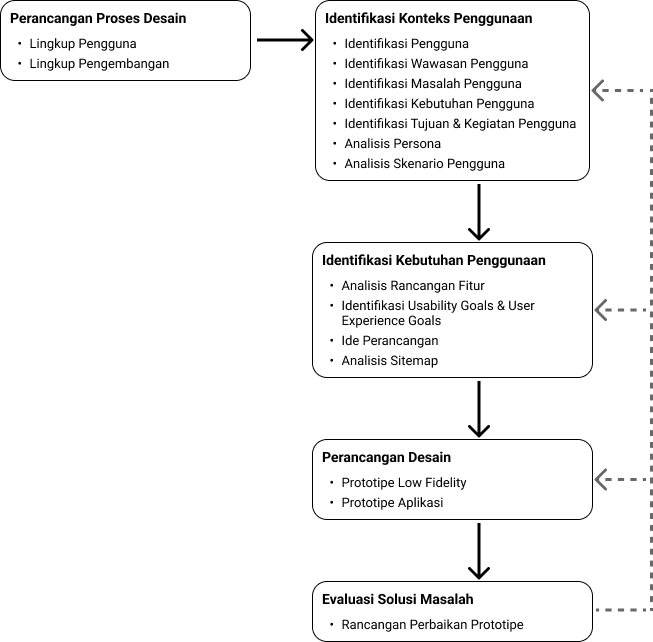
\includegraphics[width=0.8\textwidth]{chapter-3-alur-penelitian.png}
%   \caption{Alur Kerja Penelitian}
%   \label{fig:diagram_alur_kerja}
% \end{figure}

% \subsection{Perancangan Proses Desain}
% Ruang lingkup yang ditentukan pada penelitian ini adalah sebagai berikut

% \begin{enumerate}
%   \item Lingkup Pengguna
%   \subitem Target pengguna dari penelitian ini adalah masyarakat Indonesia yang pernah menggunakan atau memiliki ketertarikan terhadap aplikasi pencegah distraksi. Rentang usia dari target pengguna tidak dibatasi, namun difokuskan kepada golongan \textit{millenials} dengan rentang usia 18-30 tahun.
%   \item Lingkup Pengembangan
%   \subitem Desain interaksi aplikasi pencegah distraksi yang dibuat memiliki bentuk \textit{mobile interface} dengan mewujudkan sebuah prototipe aplikasi dalam \textit{platform Android}. Aplikasi Digital Wellbeing milik Google ditetapkan menjadi garis dasar pengembangan prototipe aplikasi tersebut.
% \end{enumerate}


% \subsection{Identifikasi Konteks Penggunaan}

% Pada tahap ini dilakukan analisis hasil riset penggunaanalisis terhadap hasil riset yang


% \subsection{Identifikasi Kebutuhan Pengguna}


% \subsection{Perancangan Desain}


% \subsection{Evaluasi Solusi Masalah}



% % Ketiga solusi yang telah diuraikan pada subbab \ref{sec:analisis_solusi} akan diimplementasikan dalam prototipe aplikasi, beserta fitur-fitur lain pada Digital Wellbeing yang akan mendukung solusi tersebut. Prototipe aplikasi ini akan diimpementasikan pada \textit{platform} Android. Secara garis besar, proses perancangan prototipe aplikasi akan menggunakan pendekatan \textit{user-centered design} (UCD).

% Seperti yang telah disebutkan pada subbab \ref{sec:metodologi}, metodologi yang digunakan dalam pengerjaan Tugas Akhir ini akan menggunakan pendekatan UCD. Dengan maksud mengikuti prosesnya, maka langkah selanjutnya yang akan dilakukan adalah mengumpulkan data. Pengumpulan data akan dilakukan dengan menyebarkan form secara online serta melakukan wawancara dengan responden yang bersedia untuk bekerja sama lebih lanjut. Proses ini akan dilaksanakan pada periode pengerjaan Tugas Akhir 2. Pengumpulan data ini bertujuan untuk melakukan validasi terhadap permasalahan yang sudah dianalisis, dan juga tidak menutup kemungkinan untuk menemukan permasalahan desain interaksi lain dari masukan pengguna.

% Setelah melakukan pengumpulan data, akan dilakukan analisis terhadap masukan yang didapat untuk mejadi kebutuhan perangkat lunak. Hasil analisis juga akan memvalidasi analisis masalah dan solusi yang didapat dari observasi penulis pada subbab \ref{sec:analisis_masalah} dan \ref{sec:analisis_solusi}.

% Kebutuhan perangkat lunak yang telah disusun akan diimplementasi dalam bentuk prototipe \textit{low-fidelity} terlebih dahulu. Setelah dilakukan evaluasi, maka implementasi akan dilanjutkan dalam bentuk prototipe \textit{high-fidelity}. Setelah menjalani evaluasi, maka perancangan prototipe aplikasi akan dikerjakan. Prototipe aplikasi diharapkan akan menghasilkan data dengan kualitas yang lebih tinggi pada saat evaluasi dibandingkan saat menggunakan prototipe \textit{low-fidelity} atau \textit{high-fidelity}. Hasil evaluasi juga akan menentukan apakah aplikasi akan menjalani proses iterasi atau diimplementasi lebih lanjut.

% \blindtext